% This file is a template using the "beamer" package to create slides for a talk or presentation
% - Talk at a conference/colloquium.
% - Talk length is about 20min.
% - Style is ornate.


% draft包的作用是在编译时不生成目录、图片、超链接等,只处理文字和排版(未显示内容用同等大小的灰色方框替代)
% 这样可以在编辑文档查看效果时加快编译速度
% 但是在确定文档内容后,需要删除draft包(使用下一行documentclass),否则目录不会生成。
% \documentclass[aspectratio=169, UTF8, draft]{beamer}
\documentclass[aspectratio=169, UTF8]{beamer}

\usepackage{ctex} % 中文支持
\usepackage{multicol} % 多栏支持
\usepackage{listings} % 代码高亮
\usetheme{Kokura}

\usepackage[english]{babel} % 在toc中显示英文

% 在封面页需要展示的信息
\title{\textbf{基于Cesium的实景三维专题表达方法研究}}
\subtitle{一份毕业答辩Beamer演示文稿示例} % 可选
\author{Falldio}
\institute{武汉大学资源与环境科学学院}
\date{2021年5月6日}

% Delete this, if you do not want the table of contents to pop up at
% the beginning of each subsection:
% \AtBeginSubsection[]
% {
  % \begin{frame}<beamer>{Outline}
    % \tableofcontents[currentsection,currentsubsection]
  % \end{frame}
% }

\begin{document}
% 默认在title page中加入图片background.png
{
  \usebackgroundtemplate{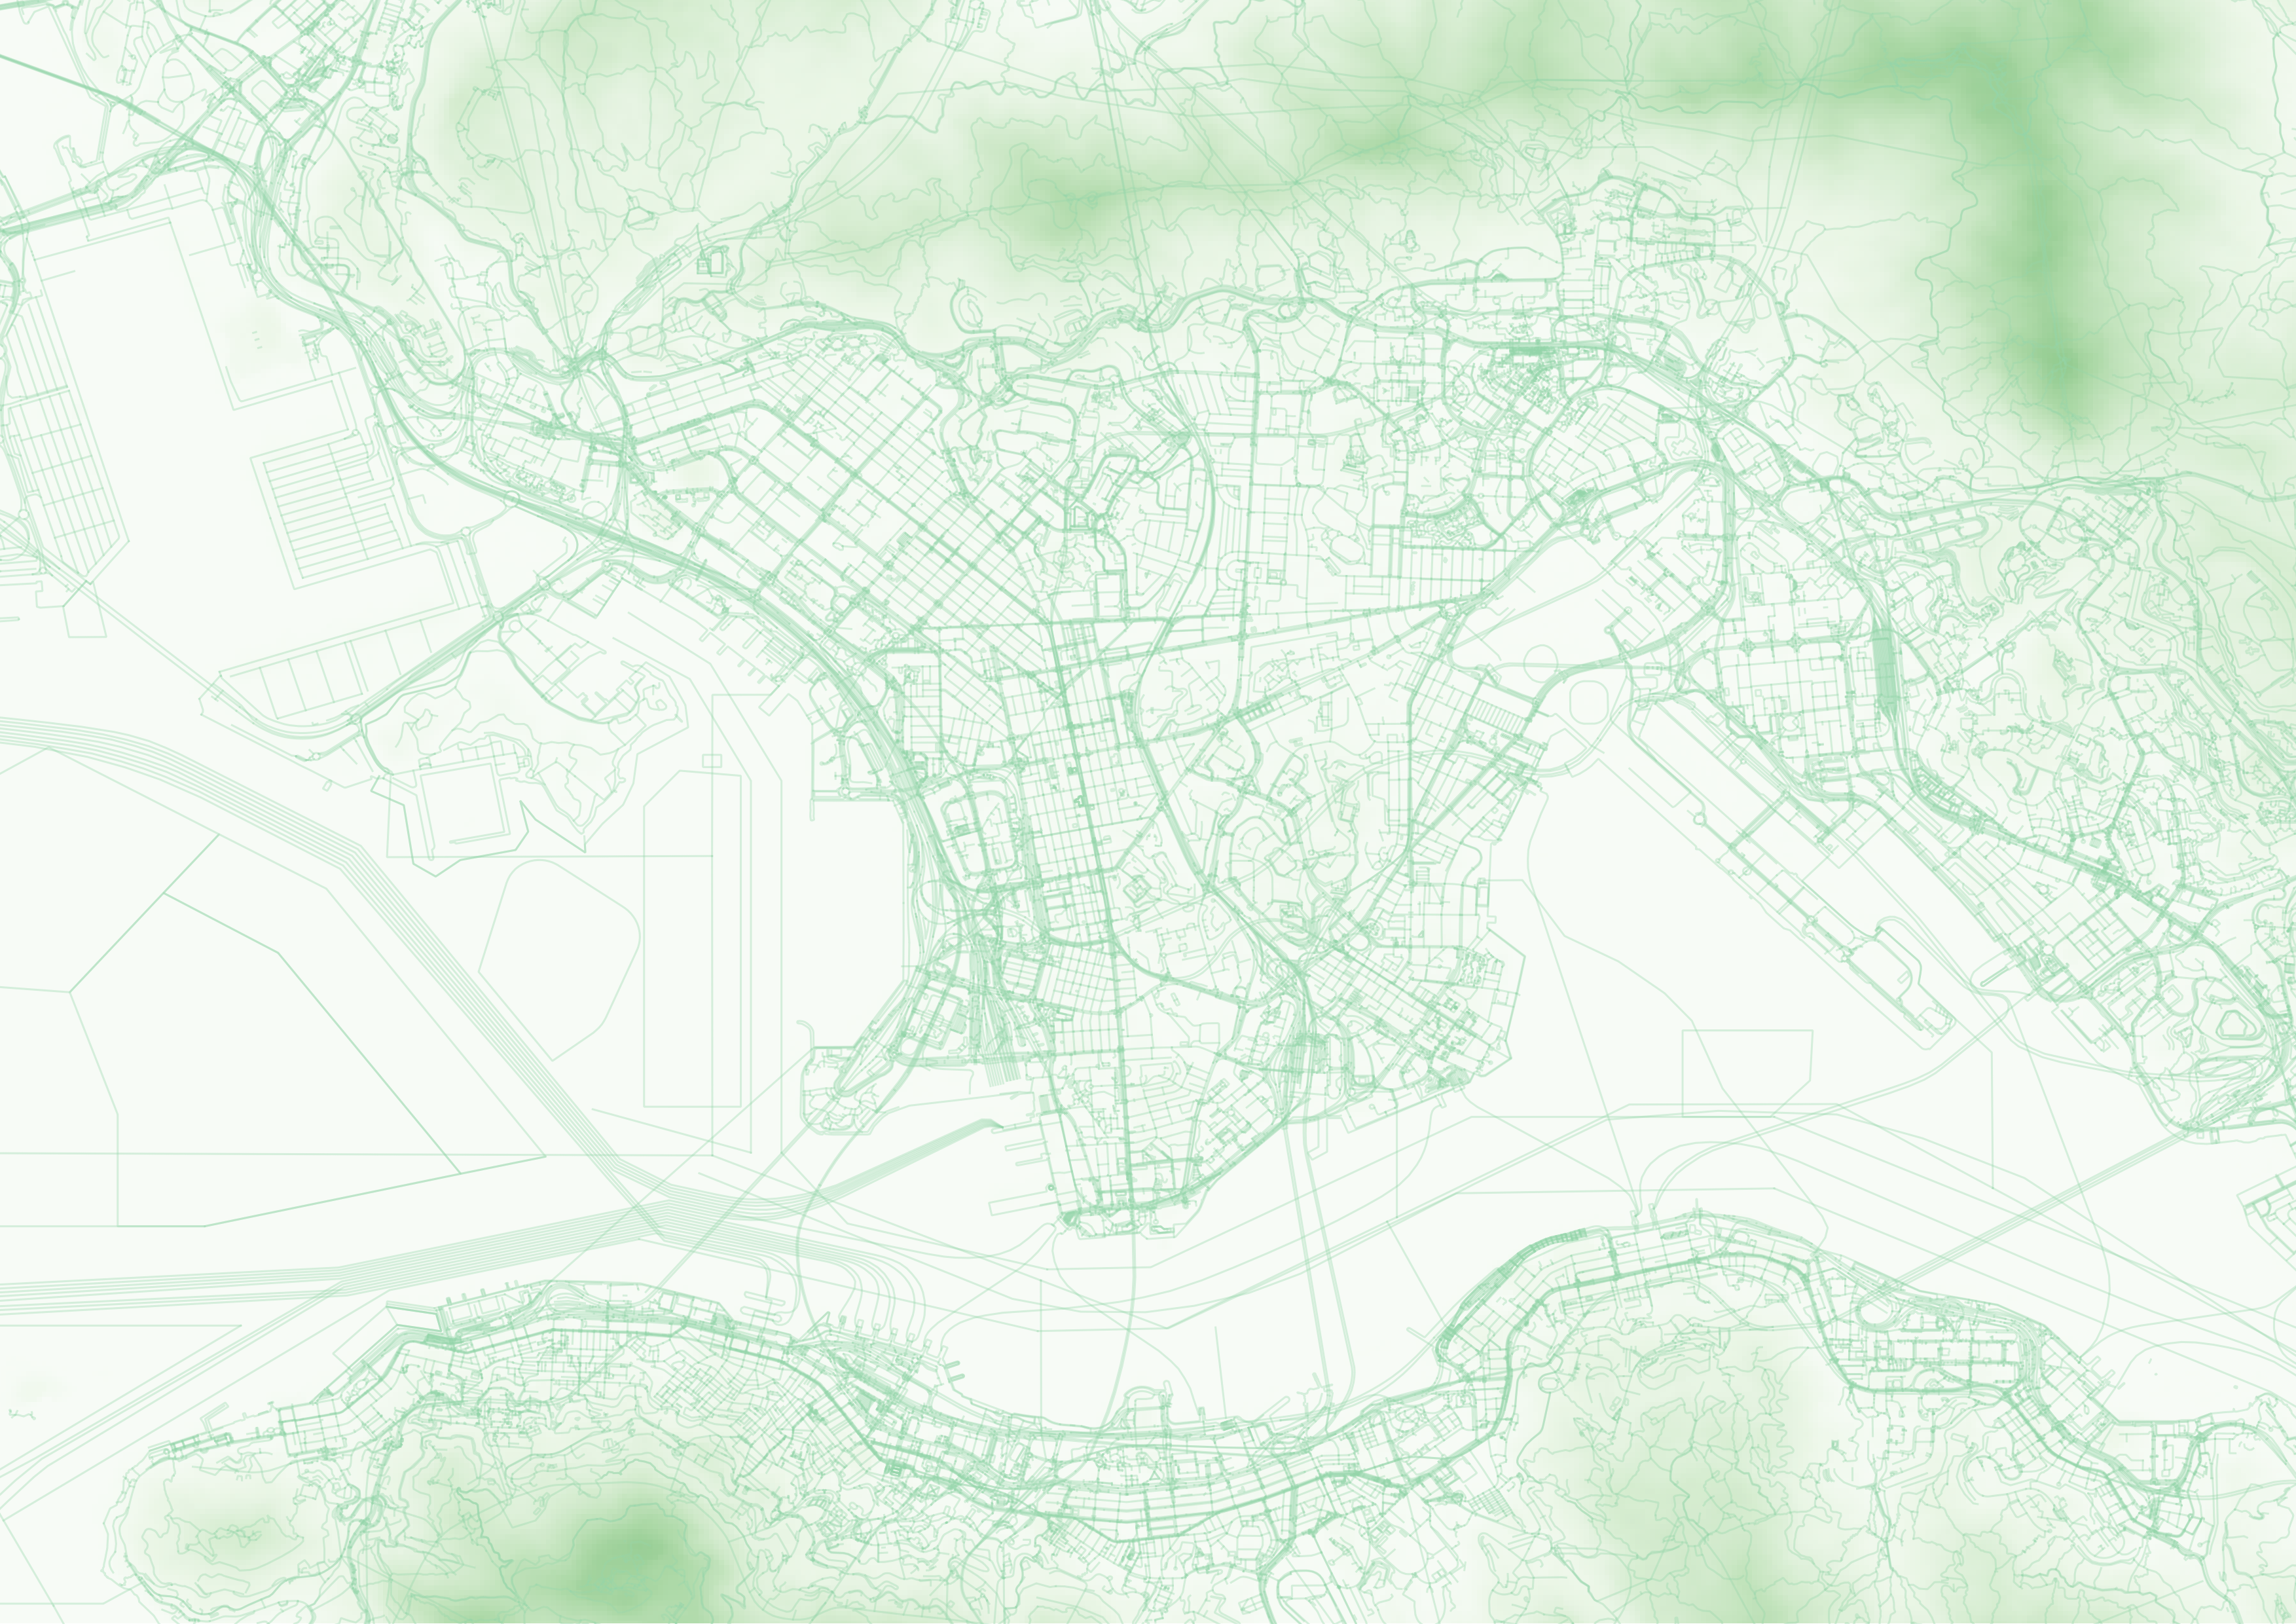
\includegraphics[width=\paperwidth]{background.png}} % 背景图片
  \begin{frame}[plain, noframenumbering]
    \titlepage
  \end{frame}
}

% 如果不需要背景图片,可以使用下面的命令
% \begin{frame}[plain, noframenumbering]
  % \titlepage
% \end{frame}

% 目录自动生成,显示所有的section和subsection
\begin{frame}[plain, allowframebreaks, noframenumbering]{目录}
  % \begin{multicols}{2} % 多栏显示
  %   \tableofcontents[]%
  % \end{multicols}
  % 如果想要单栏显示目录,可以使用下面的命令
  \tableofcontents
\end{frame}

% 内容主体
\section{研究背景}

\begin{frame}{研究背景与意义}
\end{frame}
\section{理论方法}

\subsection{分栏显示}
\begin{frame}{经典的双栏显示,一边图片一边文字}
    \begin{columns}
        \begin{column}{0.5\textwidth}
            人为分栏可通过columns语法实现\\
            双栏的宽度比例可以通过参数调整\\

        \end{column}
        \begin{column}{0.5\textwidth}
            \begin{figure}[h]
                \centering
                \includegraphics[width=0.5\textwidth]{images/example.png}
                \caption{一张简单的图片示例}
                \label{fig:3dtiles}
            \end{figure}
        \end{column}
    \end{columns}
\end{frame}

\subsection{列表}
\begin{frame}{不带编号的列表}
    使用itemize环境,使用item命令添加列表项
    \begin{itemize}
        \item 1
        \item 2
        \item 3
    \end{itemize}
\end{frame}

\begin{frame}{带有编号的列表}
    使用enumerate环境,使用item命令添加列表项
    \begin{enumerate}
        \item 1
        \item 2
        \item 3
    \end{enumerate}
\end{frame}

\subsection{数学公式}
\begin{frame}{数学公式}
    简单的数学公式使用\$...\$包裹,复杂的公式使用equation环境
    \begin{equation}
        \label{eq:1}
        \sum_{i=1}^n a_i=0
    \end{equation}
\end{frame}
\section{Experiment}

\subsection{YOLOv8 With EMA and WIoU}
\begin{frame}{Inprovement: Efficient Multi-scale Attention}
	\begin{figure}[h]
		\centering
		\includegraphics[width=0.65\textwidth]{images/ca_ema.png}
		\caption{Structure of CA and EMA}
		\label{fig:ca_ema}
	\end{figure}
\end{frame}



\begin{frame}{Inprovement: Efficient Multi-scale Attention}
	\begin{block}{Pooling output comparison}
		\begin{columns}
			\begin{column}{0.4\textwidth}
				In coordinate attention(CA), the 1D global average-pooling for encoding information along the horizontal dimension direction in $C$ at height $H$ can be denoted by
				\begin{equation}
					z^H_c(H)=\frac{1}{W}\sum_{0\leq i\leq W} x_c(H,i)
				\end{equation}
				The pooling output in $C$ at width $W$ can be formulated as
				\begin{equation}
					z^W_c(W)=\frac{1}{H}\sum_{0\leq j\leq H}x_c(j,W)
				\end{equation}
			\end{column}
			\begin{column}{0.4\textwidth}
				Efficient multi-scale attention(EMA) employs 2D global average pooling to aggregate cross-spatial information, encoding it into the $1\times 1$ branch output. Outputs of the least branch will be transformed to the correspond dimension shape before the joint activation mechanism of channel features, i.e., $\mathbb{R}^{1\times C//G}_1\times \mathbb{R}^{C//G\times HW}_3$. The 2D global pooling operation is
				\begin{equation}
					z_c=\frac{1}{H\times W}\sum^H_j\sum^W_i x_c(i,j)
				\end{equation}
			\end{column}
		\end{columns}
	\end{block}
\end{frame}

\begin{frame}{Inprovement: Wise-IoU}
	In YOLOv2, we have bounding box regression(BBR) loss expressed as
	\begin{equation}
		\mathcal{L}(\vec{B},\vec{B_{gt}})=\left|\left|\vec{B}-\vec{B_{gt}}\right|\right|
	\end{equation}
	But it cannot shield the inference of the size of the bounding box. So we come up with intersection over union(IoU)
	\begin{equation}
		\mathcal{L}_\text{IoU}=1-\text{IoU}=1-\frac{W_i H_i}{S_i}
	\end{equation}
	In order to prevent circumstances like $W_i=0$ or $H_i$, we add penalty term $\mathcal{R}_i$
	\begin{equation}
		\mathcal{L}_i=\mathcal{L}_\text{IoU}+\mathcal{R}_i
	\end{equation}
	\begin{figure}[h]
		\centering
		\includegraphics[width=0.21\textwidth]{images/iou.png}
		\caption{An IoU example}
		\label{fig:iou}
	\end{figure}
\end{frame}

\begin{frame}{Inprovement: Wise-IoU}
	\begin{columns}
		\begin{column}{0.5\textwidth}
			\begin{block}{Distance-IoU}
				Consider normalized distance between central points of two bounding boxes
				\begin{equation}
					\mathcal{R}_\text{DIoU}=\frac{\left(x-x_{g t}\right)^2+\left(y-y_{g t}\right)^2}{W_g^2+H_g^2}
				\end{equation}
			\end{block}
		\end{column}
		\pause
		\begin{column}{0.5\textwidth}
			\begin{block}{Complete-IoU}
				Add the consideration of aspect ratio
				\begin{equation}
					\mathcal{R}_\text{CIoU}=\mathcal{R}_\text{DIoU}+\alpha v,\alpha=\frac{v}{\mathcal{L}_\text{IoU}+v}
				\end{equation}
			\end{block}
		\end{column}
	\end{columns}
\end{frame}

\begin{frame}{Inprovement: Wise-IoU}
	\begin{columns}
		\begin{column}{0.45\textwidth}
			\begin{block}{Efficient-IoU}
				Increase the punishment for distance metric
				\begin{equation}
					\mathcal{R}_\text{EIoU}=\mathcal{R}_\text{DIoU}+\frac{\left(x-x_{g t}\right)^2}{W_g^2}+\frac{\left(y-y_{g t}\right)^2}{H_g^2}
				\end{equation}
			\end{block}
		\end{column}
		\pause
		\begin{column}{0.55\textwidth}
			\begin{block}{Scylla-IoU}
				We define angle cost as
				\begin{equation}
					\Lambda=\sin \left(2 \sin ^{-1} \frac{\min \left(\left|x-x_{g t}\right|,\left|y-y_{g t}\right|\right)}{\sqrt{\left(x-x_{g t}\right)^2+\left(y-y_{g t}\right)^2}+\varepsilon}\right)
				\end{equation}
				Then the distance cost comes to be
				\begin{equation}
					\Delta=\frac{1}{2} \sum_{t=w, h}\left(1-e^{-\gamma \rho_t}\right), \gamma=2-\Lambda
				\end{equation}
				Therefore, we have
				\begin{equation}
					\mathcal{R}_\text{SIoU}=\Delta+\Sigma
				\end{equation}
			\end{block}
		\end{column}
	\end{columns}
\end{frame}

\begin{frame}{Inprovement: Wise-IoU}
	\begin{block}{Wise-IoU}
		Based on SIoU and EIou, we reconsider low-quality examples and geometric factors, and construct Wise-IoU with 2 layers of attention mechanism
		\begin{equation}
			\mathcal{L}_\text{WIoU}=\mathcal{R}_\text{WIoU}\mathcal{L}_\text{IoU}
		\end{equation}
		where
		\begin{equation}
			\mathcal{R}_\text{WIoU}=\exp\left(\frac{(x-x_{gt})^2+(y-y_{gt})^2}{(W^2_g+H^2_g)^*}\right)
		\end{equation}
		$\mathcal{R}_\text{WIoU}\in [1,e)$ which will significantly amplify $\mathcal{L}_\text{IoU}$ of the ordinary-quality anchor box. $\mathcal{L}_\text{IoU}\in [0,1]$, which will significantly reduce $\mathcal{R}_\text{WIoU}$ of the high-quality anchor box and its focus on the distance between central points when the anchor box coincides well with the target box.\\
		Superscript $*$ indicates $W_g,H_g$ are detached from the computational graph.
	\end{block}
\end{frame}

\begin{frame}{Experiment: Where to add EMA?}
	\begin{figure}[h]
		\centering
		\includegraphics[width=\textwidth]{images/ema_add.png}
		\caption*{}
	\end{figure}
\end{frame}

\begin{frame}{Experiment: How's the combination?}
	\begin{figure}[h]
		\centering
		\includegraphics[width=\textwidth]{images/improve_combination.png}
		\caption*{}
	\end{figure}
\end{frame}

\begin{frame}{Assessment: EMA and WIoU}
	\begin{figure}[h]
		\centering
		\includegraphics[width=\textwidth]{images/loss_1.png}
		\caption{Results}
		\label{fig:loss1}
	\end{figure}
\end{frame}

\begin{frame}{Assessment: EMA and WIoU}
	\begin{columns}
		\begin{column}{0.5\textwidth}
			\begin{figure}[h]
				\centering
				\includegraphics[width=0.87\textwidth]{images/confusion_origin.png}
				\caption{Original YOLOv8 confusion matrix}
				\label{fig:confusion_origin}
			\end{figure}
		\end{column}
		\begin{column}{0.5\textwidth}
			\begin{figure}[h]
				\centering
				\includegraphics[width=0.85\textwidth]{images/confusion_improve.png}
				\caption{Improved YOLOv8 confusion matrix}
				\label{fig:confusion_improve}
			\end{figure}
		\end{column}
	\end{columns}
\end{frame}

\begin{frame}{Results: EMA and WIoU}
	\begin{columns}
		\begin{column}{0.5\textwidth}
			\begin{figure}[h]
				\centering
				\includegraphics[width=0.7\columnwidth]{images/origin.jpg}
				\caption{Original labels}
%				\includegraphics[width=0.45\columnwidth]{images/yolov8.jpg}
%				\caption{YOLOv8 segmentation}
			\end{figure}
		\end{column}
		\begin{column}{0.5\textwidth}
			\begin{figure}[h]
%				\includegraphics[width=0.45\columnwidth]{images/ema_backbone.jpg}
%				\caption{YOLOv8 with EMA segmentation}
				\includegraphics[width=0.7\columnwidth]{images/ema_wiou.jpg}
				\caption{YOLOv8 with EMA and WIoU segmentation}
			\end{figure}
		\end{column}
	\end{columns}
\end{frame}

\subsection{Deep Snake, Flexible Design}
\begin{frame}{Inprovement: Deep Layer Aggregation}
	\begin{figure}[h]
		\centering
		\includegraphics[width=0.9\textwidth]{images/diff_aggregation.pdf}
		\caption{Different ways to aggregate layers}
		\label{fig:diff_aggregation}
	\end{figure}
\end{frame}

\begin{frame}{Inprovement: Deep Layer Aggregation}
	\begin{figure}[h]
		\centering
		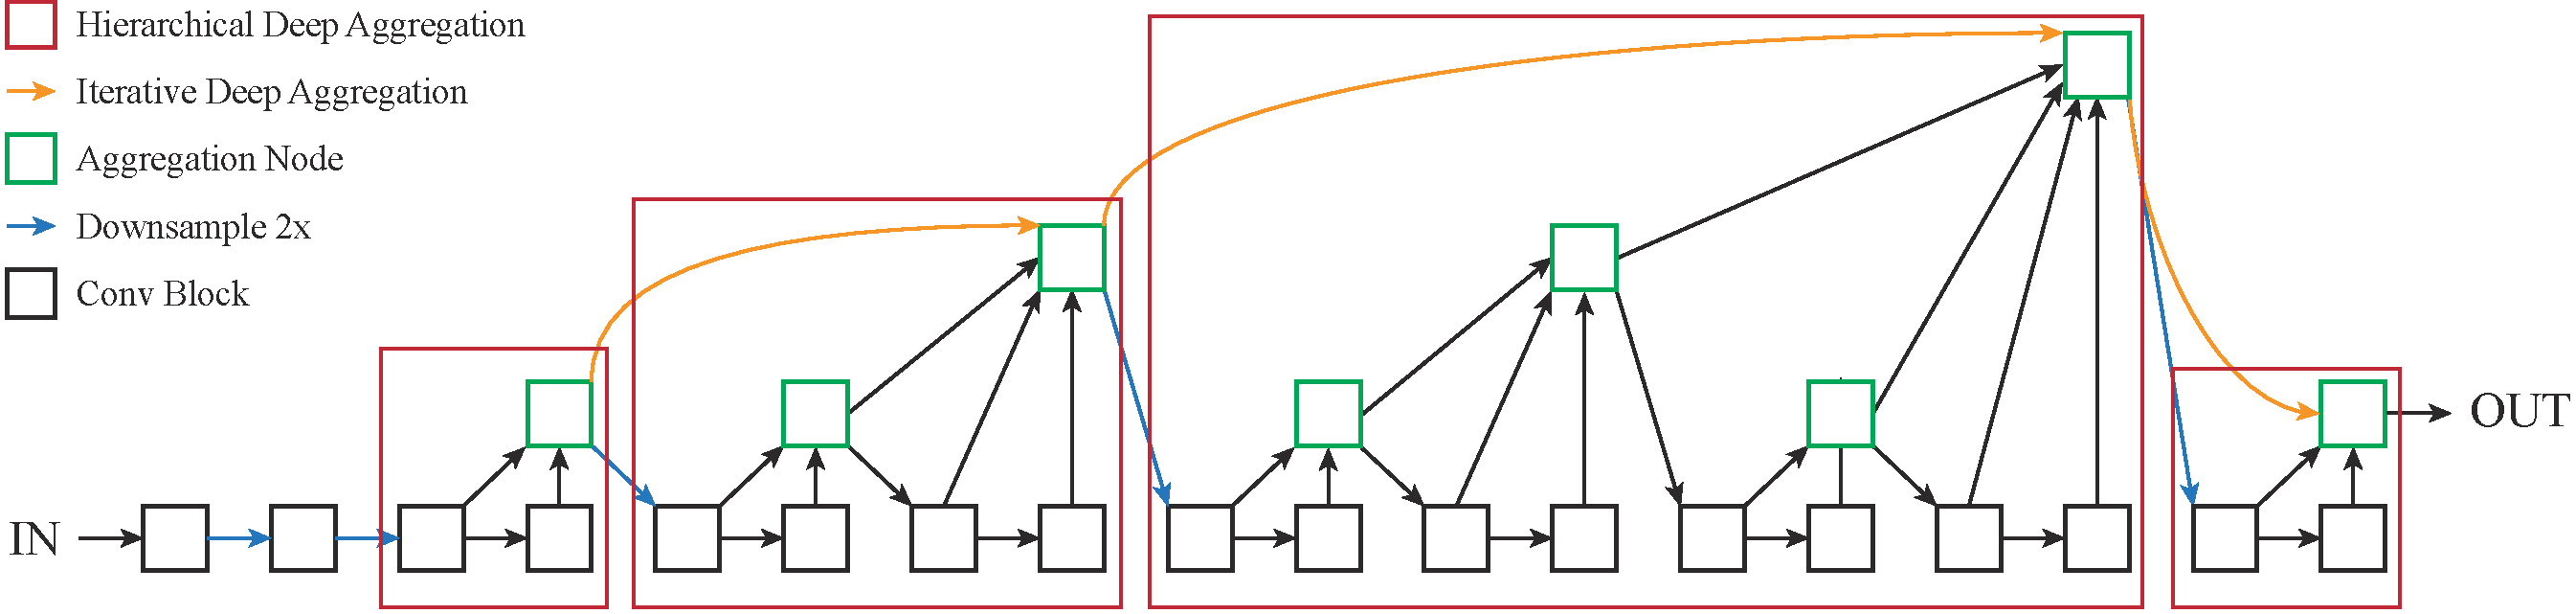
\includegraphics[width=\textwidth]{images/dla_architecture.pdf}
		\caption{DLA network architecture}
		\label{fig:dla_architecture}
	\end{figure}
\end{frame}

\begin{frame}{Experiment: Deep Snake}
	\begin{figure}[h]
		\centering
		\includegraphics[width=0.7\textwidth]{images/train_loss.png}
		\caption{Loss during training}
		\label{fig:train_loss}
	\end{figure}
\end{frame}

\begin{frame}{Experiment: Deep Snake}
	\begin{figure}[h]
		\centering
		\includegraphics[width=0.7\textwidth]{images/val_loss.png}
		\caption{Loss during validation}
		\label{fig:val_loss}
	\end{figure}
\end{frame}

\begin{frame}{Experiment: Deep Snake}
	\begin{figure}[h]
		\centering
		\includegraphics[width=0.8\textwidth]{images/deepsnake_demo.png}
		\caption{Sample pictures segmented by Deep Snake}
		\label{fig:deepsnake_demo}
	\end{figure}
\end{frame}
\section{总结展望}

\begin{frame}{总结展望}
\end{frame}

% 致谢页面
{
    \usebackgroundtemplate{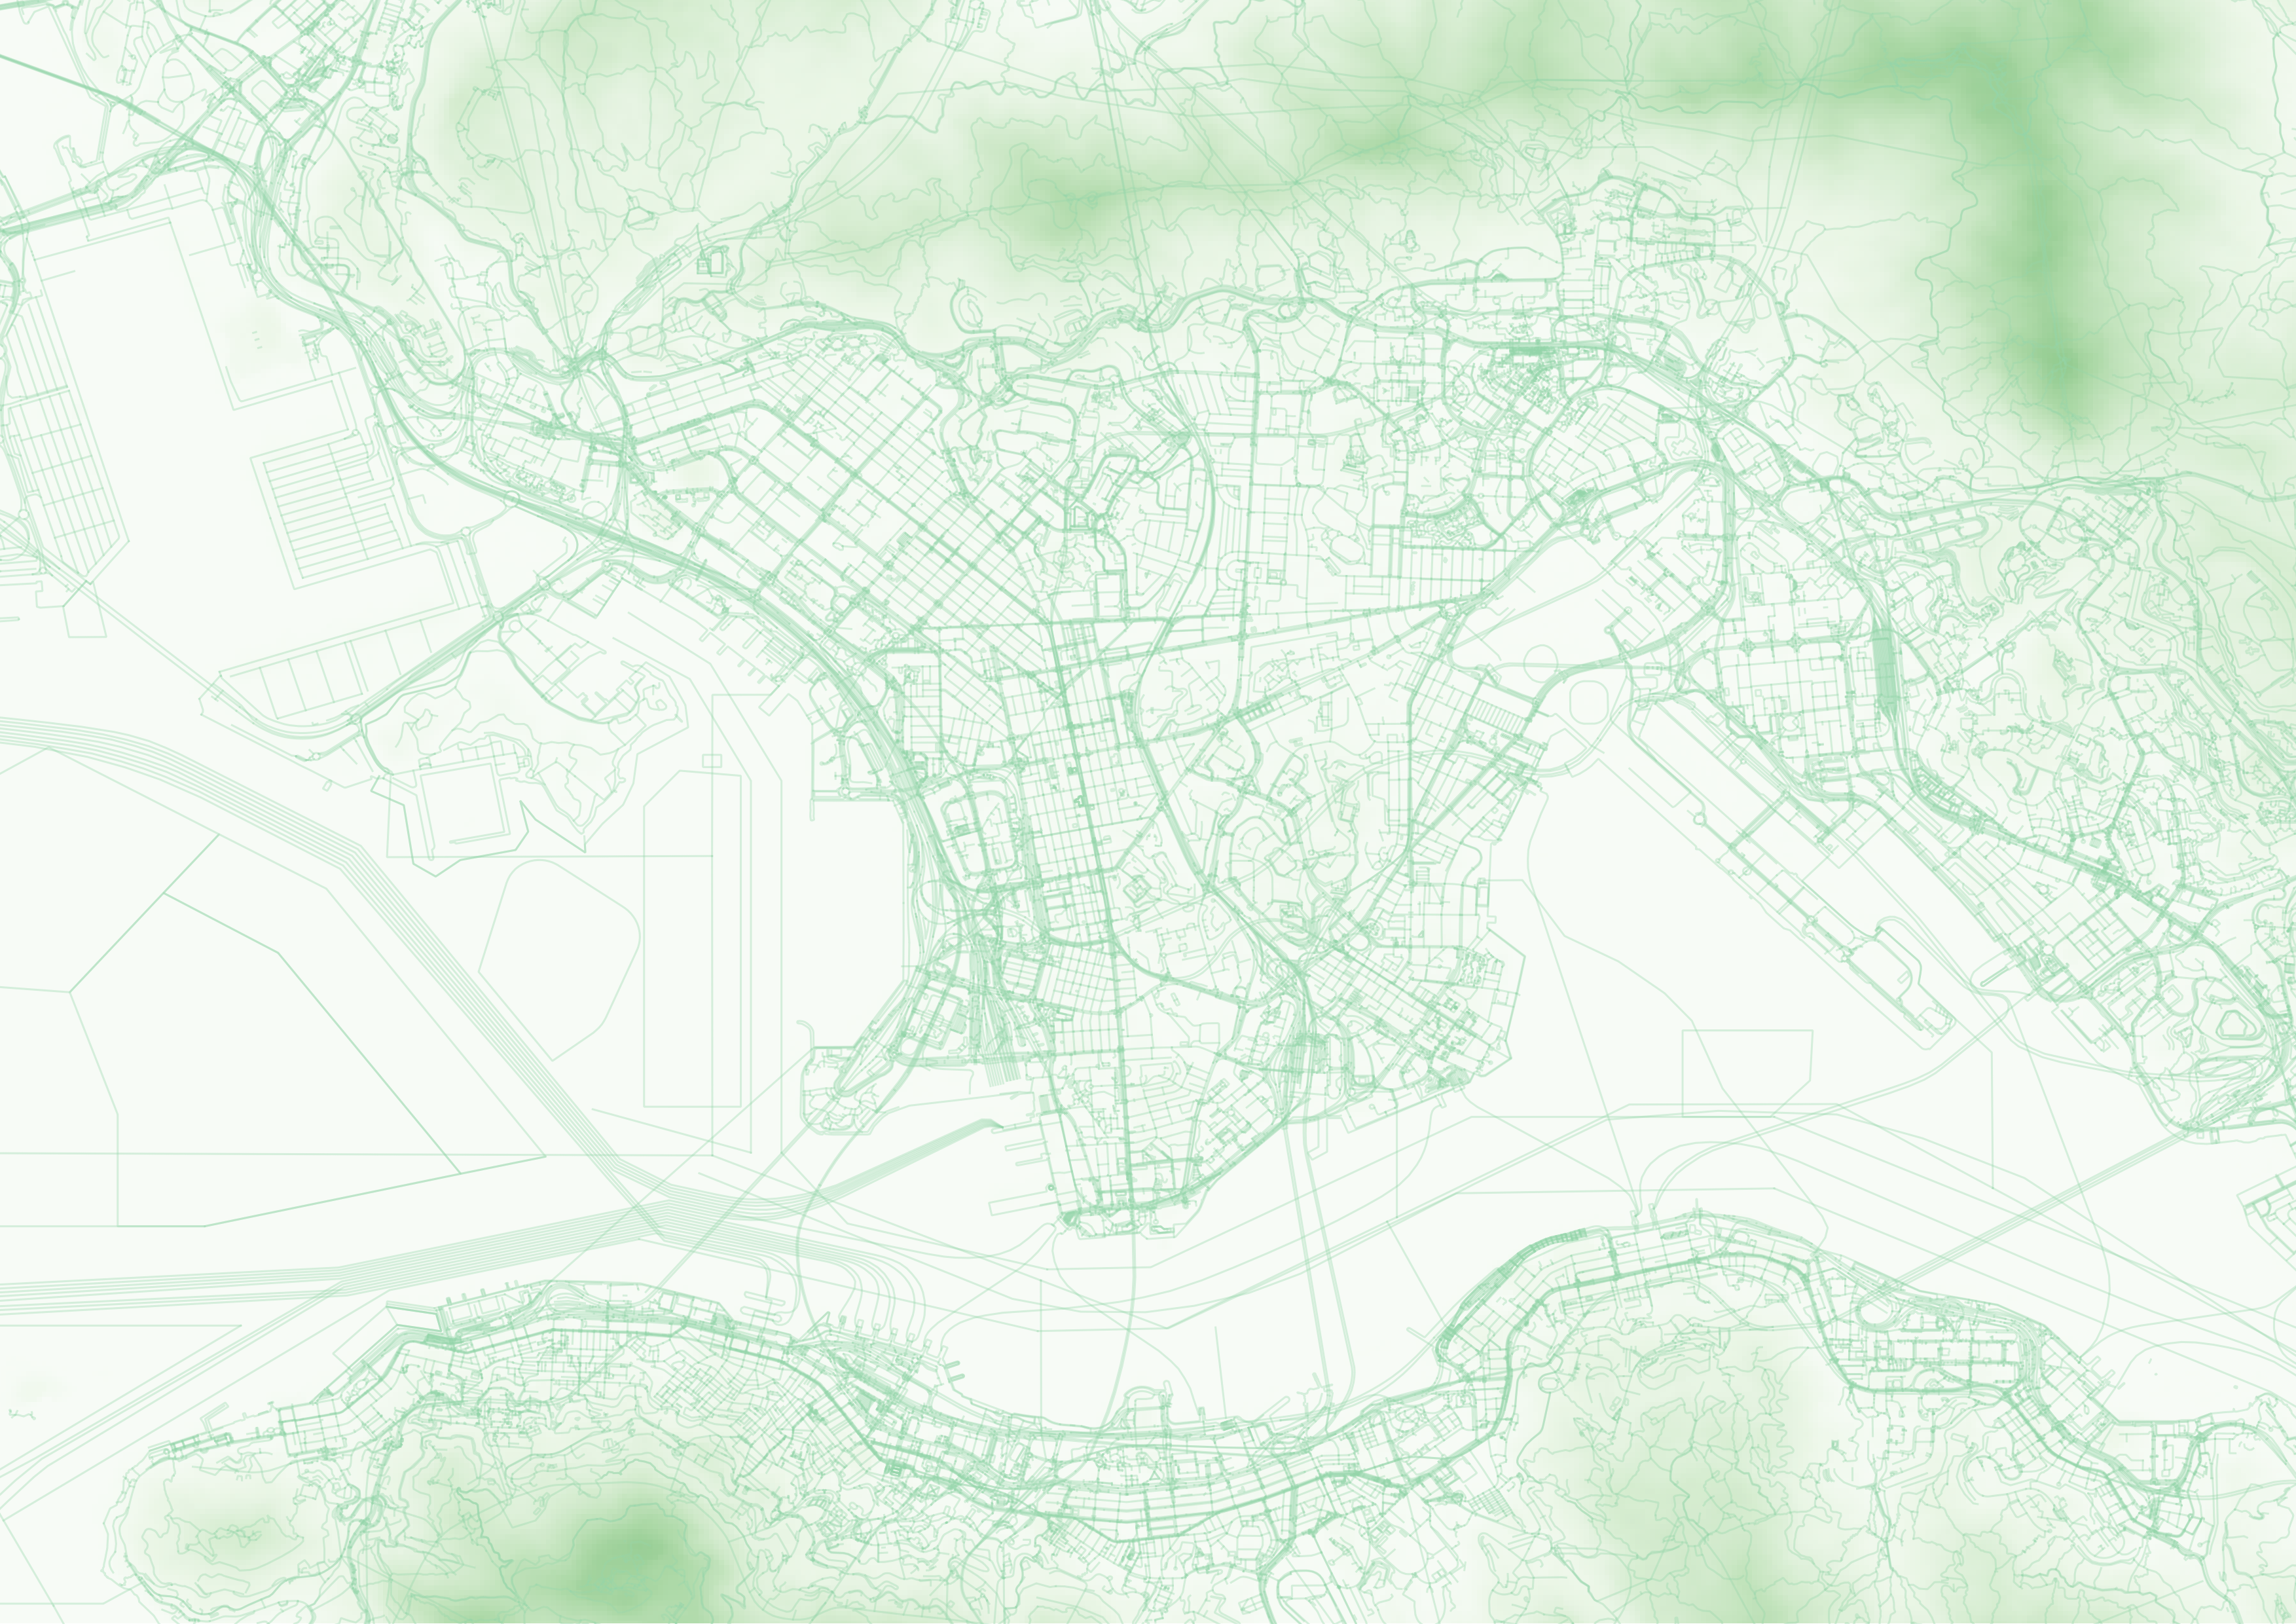
\includegraphics[width=\paperwidth]{background.png}} % 背景图片
    \usebeamercolor{structure}
    \begin{frame}[plain]
        \begin{center}
            \textcolor{fg}{\Huge \textbf{敬请各位老师批评指正!}}
            \vskip 1cm
            \textcolor{fg}{\large 焚膏油以继晷,恒兀兀以穷年。}
        \end{center}
    \end{frame}
}

\end{document}


